\documentclass[../tfg.tex]{subfiles}

\begin{document}

\section{CVE-2021-3156}
\label{example:baron_samedit}
On 2021-01-26, the Qualys Research Team disclosed a vulnerability on the \texttt{sudo} command that allowed privilege escalation via heap overflow\cite{qualys:baron_samedit}.

The \texttt{sudo} program is a utility for UNIX systems that allows a user to run programs with the privileges of another user. It comes installed by default in almost all Linux distributions.

The affected versions go from 1.8.2 to 1.8.31p2 for legacy versions and from 1.9.0 to 1.9.5p1 for stable versions. Exploits have been tested for Ubuntu 20.04, Debian 10, Fedora 33, MacOS Big Sur.

\subsection{Weakness}
The weakness exploited is an \textbf{off-by-one error} (\href{https://cwe.mitre.org/data/definitions/193.html}{CWE-193}). That means that the range for a loop is wrongly calculated to do more iterations than intended.
\begin{lstlisting}[caption={Example of off-by-one}]
char from[] = {0x41, 0x41, 0x41, 0x41, '\\', 0x0, 0x41, 0x41, 0x0};
char* to = malloc(sizeof(char) * strlen(from) + 1);

while(*from)
{
    if(from[0] == '\\')
        from++;
    *to++ = *from++;
}
\end{lstlisting}

\subsection{Bug}
\subsubsection{Vulnerability identification}
In \texttt{set\_cmnd()} heap overflow could happen if a command line argument ends with a backslash. A buffer is allocated on the heap to store the user provided arguments. To know the length of the buffer it iterates over \texttt{argv} and calls \texttt{strlen} that stops on a null termination byte. \textbf{By changing the arguments provided to \texttt{sudo} we can control the size of the heap allocated buffer.}
\begin{lstlisting}[caption={\texttt{sudoers.c:set\_cmnd}}]
size_t size, n;

/* Alloc and build up user_args. */
for (size = 0, av = NewArgv + 1; *av; av++)
    size += strlen(*av) + 1;

if (size == 0 || (user_args = malloc(size)) == NULL) {
    sudo_warnx(U_("%s: %s"), __func__, U_("unable to allocate memory"));
    debug_return_int(-1);
}
\end{lstlisting}
Later, the program rewrites the \texttt{argv} values on the newly allocated buffer. But inside the transferring code there is an \textbf{off-by-one} bug hidden. By providing a backslash on the input we can make the \texttt{from} pointer advance two positions on an iteration, \textbf{jumping over the null byte that would stop the copying}.

\begin{figure}[H]
    \centering
    \subfile{../imgs/examples/baron_samedit/out_of_bounds_arg.tex}
    \caption{Out-of-bounds access}
\end{figure}

\begin{enumerate}
    \item While \texttt{*from} is different from \texttt{0x0} keep looping
    \begin{enumerate}
        \item \texttt{from[0]} points to the backslash and \texttt{from[1]} points to the null termination byte.
        \begin{enumerate}
            \item \texttt{from} gets incremented and now points to the null termination byte, skipping over the backslash.
        \end{enumerate}
        \item The null byte is copied into the buffer and \texttt{from} gets incremented. Now \texttt{from} is pointing to the data \textbf{after} the null byte.
    \end{enumerate}
\end{enumerate}

This way, the \texttt{while} loop will copy more data than was previously calculated, writing outside of the heap allocated buffer and overwriting critical data on the heap chunks.

\subsubsection{Reaching the vulnerable code}
\texttt{sudo} works by setting a mode of operation based on how the user invoked the command. Different modes of operation trigger execute different parts of the code. To trigger the vulnerable code, the following condition for the \texttt{sudo} mode must be set.
$$ \texttt{MODE\_SHELL} \wedge (\texttt{MODE\_EDIT} \vee \texttt{MODE\_CHECK}) \wedge \neg \texttt{MODE\_RUN}$$

\texttt{MODE\_RUN} must be turned off because it will trigger code that escapes special characters on the command line arguments. That obviously will prevent us from triggering the bug.


\texttt{MODE\_EDIT} or \texttt{MODE\_CHECK} are set manually via command line options, \texttt{-e} and \texttt{-e}, a check on \texttt{parse\_args()} turns off \texttt{MODE\_SHELL}. But calling \texttt{sudoedit} instead of \texttt{sudo} automatically sets \texttt{MODE\_EDIT} without unsetting \texttt{MODE\_SHELL}.


\texttt{MODE\_SHELL} can be set via command line option \texttt{-s}.


Therefore, by calling \texttt{sudoedit -s} we can reach the vulnerable code.

\begin{figure}[H]
    \centering
    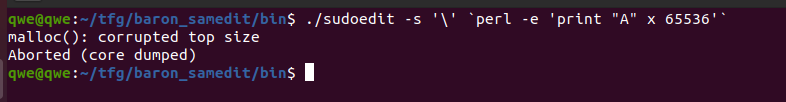
\includegraphics[width=\linewidth]{imgs/examples/baron_samedit/sudoedit_crash.png}
    \caption{Unpatched \texttt{sudo} behaviour}
\end{figure}

\begin{figure}[H]
    \centering
    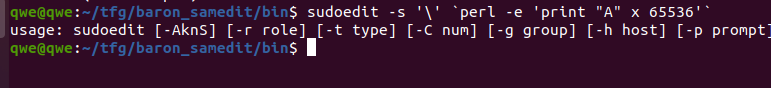
\includegraphics[width=\linewidth]{imgs/examples/baron_samedit/sudoedit_patched.png}
    \caption{Patched \texttt{sudo} behaviour}
\end{figure}

\subsection{Exploitation}
\subsubsection{Overflowing with data}
Once we know we can overflow the heap buffer, we need targets. In their report, the Qualys team first tried to abuse locale related settings to turn the buffer overflow into a format string vulnerability. In the process they implemented a fuzzer to play around with \texttt{LC\_x} environment variables. The initial plan ended up failing ultimately but thanks to the fuzzer they produced dozens of unique crashes, from which they exploited three cases.

Here I am going to discuss an implementation for the second case they presented: overwriting the name of a library loaded at runtime.

\begin{figure}[H]
    \centering
    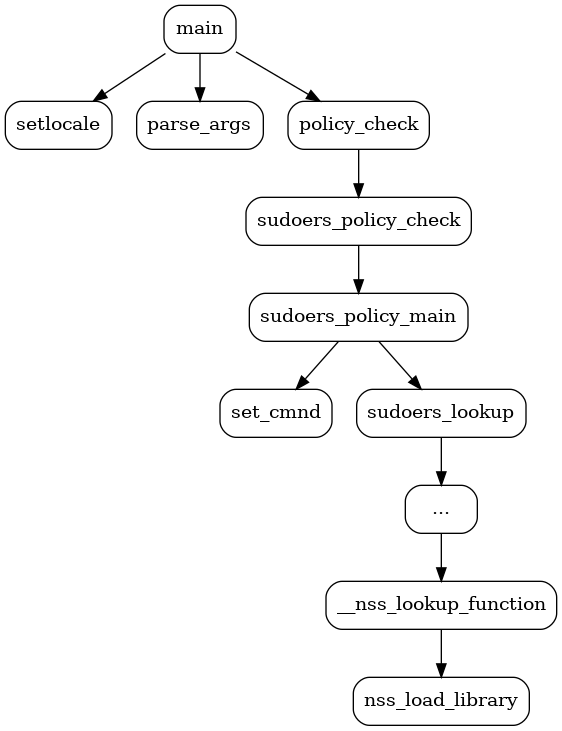
\includegraphics[scale=0.4]{imgs/examples/baron_samedit/call_graph.png}
    \caption{Relevant calls in \texttt{sudo}}
\end{figure}

\subsubsection{Name Service Switch}
NSS is a name resolution mechanism for UNIX-like systems. It is based on a group of databases that contain information about certain names.

Sudo uses this mechanism to check for permissions.

\begin{lstlisting}[caption={sudoers.c}]
cmnd_status = set_cmnd();
/* ... */
validated = sudoers_lookup(snl, sudo_user.pw, FLAG_NO_USER | FLAG_NO_HOST, pwflag);
\end{lstlisting}
Then \texttt{sudoers\_lookup} starts a chain of calls that arrives at \href{https://elixir.bootlin.com/glibc/glibc-2.31/source/nss/nsswitch.c#L401}{\texttt{\_\_nss\_lookup\_function}}.\\
\texttt{\_\_nss\_lookup\_function} calls \href{https://elixir.bootlin.com/glibc/glibc-2.31/source/nss/nsswitch.c#L328}{\texttt{nss\_load\_library}}, that loads a library specified by a name as it was a dynamically linked library with \texttt{\_\_libc\_dlopen}.
Because all these structures are allocated in the heap we can load an attacker controlled library by overwriting the \texttt{name} field of a service with the heap overflow on \texttt{set\_cmnd}.

\begin{figure}[H]
    \centering
    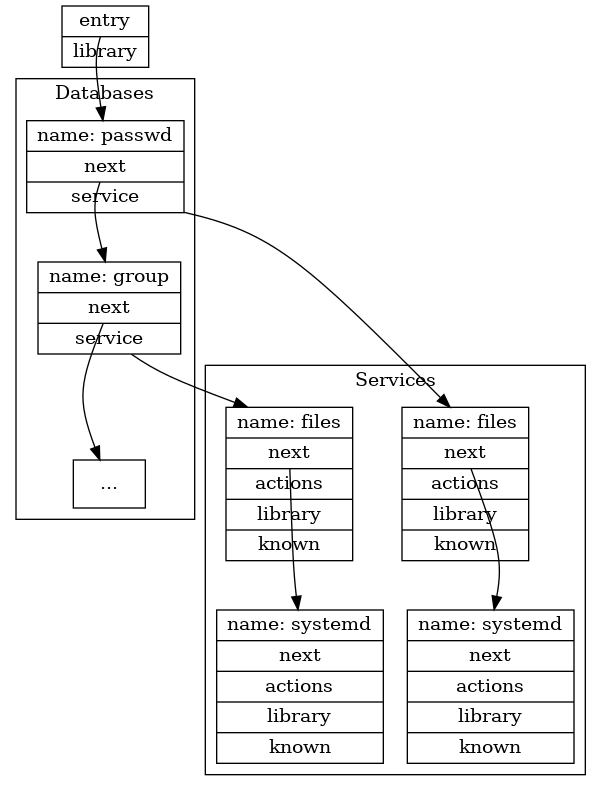
\includegraphics[height=0.5\textheight]{imgs/examples/baron_samedit/nss_structs.png}
    \caption{NSS data structures}
\end{figure}

In this case, \texttt{sudo} will try to load the service \textbf{files} from the database \textbf{group}. If we overwrite the \texttt{name} field of the service structure we will control what library \texttt{sudo} is going to load. To make sure we do not override anything that could cause a segmentation fault before \texttt{nss\_load\_library} is called we need to allocate the user input buffer closely to the chunk where this data structure is allocated. To ensure we get the chunk we want, we need to employ a special technique: \textbf{heap feng shui}.

\begin{lstlisting}
typedef struct service_user
{
  /* And the link to the next entry.  */
  struct service_user *next;
  /* Action according to result.  */
  lookup_actions actions[5];
  /* Link to the underlying library object.  */
  service_library *library;
  /* Collection of known functions.  */
  void *known;
  /* Name of the service (`files', `dns', `nis', ...).  */
  char name[0];
} service_user;
\end{lstlisting}

\subsubsection{Heap feng shui}
This technique aims to modify and influence the heap layout. Thanks to the defragmentation routines of the allocator's implementation and certain tables for reusing previously allocated chunks the heap is very dynamic in its layout. By allocating chunks of certain sizes and freeing them, we can force posterior allocations to use the previous chunks instead of creating new ones and vice versa. We just need to find the correct sizes to enforce a certain layout, one layout that is favorable to the attacker. The goal for this exploit is to set a chunk as the first chunk in any of the tcache's lists. This chunk is special in the sense that it is the previous chunk after the chunk where the \emph{group:files} NSS service is allocated. This layout must be accomplished just right before the allocation of \texttt{user\_args} in \texttt{set\_cmnd}. We can claim this chunk with a user input with the same size as the tcache's list where it is located.

\begin{figure}[H]
    \centering
    \subfile{../imgs/examples/baron_samedit/user_args_malloc.tex}
    \caption{Intended heap layout}
\end{figure}

Now, we need to find some code that we can control to make all the allocations and frees needed to shake the heap around. \texttt{setlocale} is a function used to set locale and language related settings for ease of translation at runtime. It turns out that \texttt{setlocale} performs quite a lot of \texttt{malloc}s and {free}s with environment variables used for locale settings: \texttt{LC\_CTYPE}, \texttt{LC\_TIME}, \texttt{LC\_MONETARY}, just to name a few. Because they are environment variables we can control their size and their contents, just what we needed to implement the heap feng shui technique.

I wrote a bruteforcer that will play around with the values for \texttt{LC\_*} variables and observe the state of the heap and the tcache. If the tcache holds a chunk ready to be allocated that is before the chunk where \emph{group:files} is allocated then a solution is found.

\begin{figure}[H]
\begin{minipage}[c]{0.48\linewidth}
    \centering
    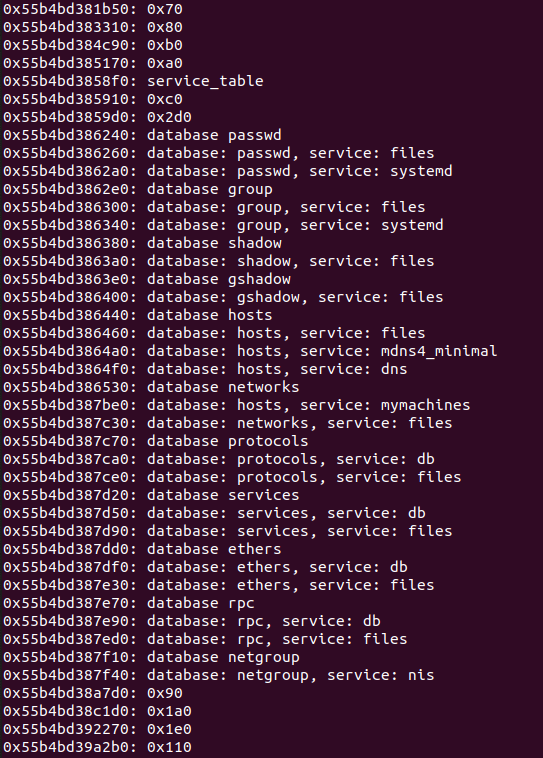
\includegraphics[width=\linewidth]{imgs/examples/baron_samedit/brute_1.png}
\end{minipage}
\begin{minipage}[c]{0.48\linewidth}
    \centering
    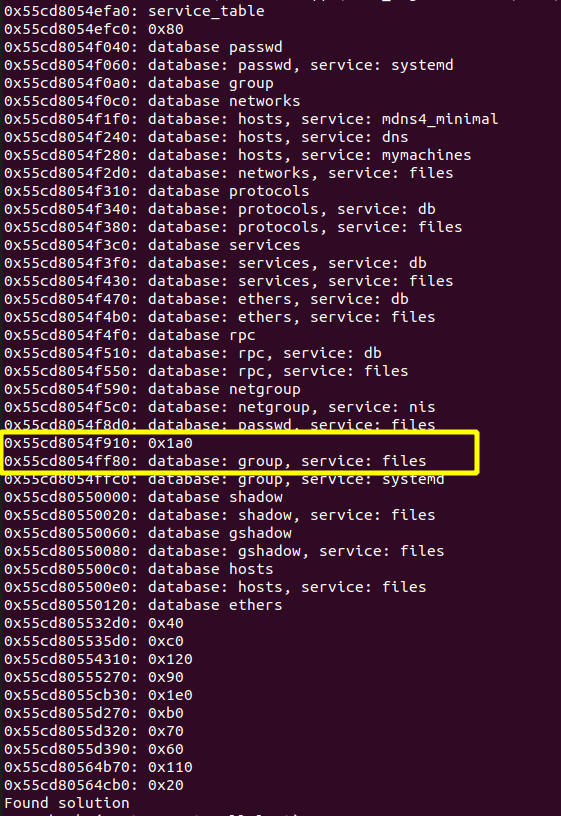
\includegraphics[width=\linewidth]{imgs/examples/baron_samedit/brute_2.png}
\end{minipage}

    \caption{Printing the heap layout while bruteforcing}
\end{figure}

\subsubsection{Overwriting with environment variables}

Now that we got our desired chunk, we just need to overflow it with data. Because we already used the user input to set the size of the chunk we wanted from the tcache we need to find another way in for the extra data.
Revisiting the \texttt{set\_cmnd}, on the lines where the overflow happens, taking a look at the variables \texttt{from}, we can see it is a pointer into the stack, where the C runtime environment puts the arguments supplied to the command. Further down the stack (towards the higher addresses) the C runtime also puts the environment variables, being adjacent to the arguments.

%\begin{figure}[H]
    %\centering
    %\subfile{../imgs/examples/baron_samedit/main_stack_frame.tex}
    %\caption{\texttt{main}'s stack frame}
%\end{figure}

This means that the \texttt{from} variable will point to the environment variables. There is where we want to put the payload for the overflow.

\begin{figure}[H]
    \centering
    \subfile{../imgs/examples/baron_samedit/overflow.tex}
    \caption{Overflow}
\end{figure}

First we need some padding to compensate for the offset where the actual data of the chunk starts versus where the chunk starts. Then we can set the new contents for the \emph{group:files} service. Lastly, put the \texttt{LC\_*} variables that the bruteforcer found as a solution.


\subsubsection{Evil library}
For the hijacked library, we are going to make a dynamically linked library that calls \texttt{execve("/bin/sh")} on the constructor. When the library gets loaded, it will automatically start execution of the constructor function and open a root shell for us. It is important for the library to be present at the same directory the exploit is executed and to be inside a folder called \texttt{libnss\_\$\{name\}}, where \texttt{name} is the name of the library.

\begin{figure}[H]
    \centering
    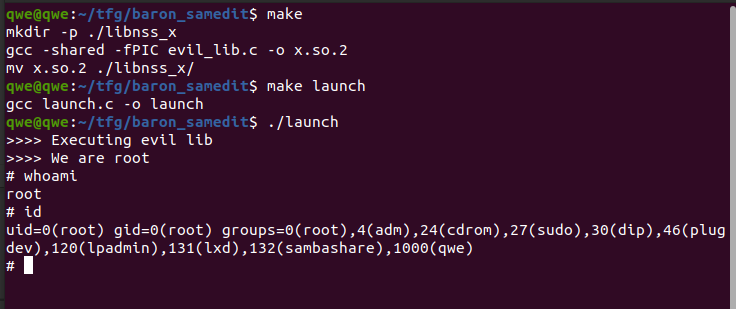
\includegraphics[width=\linewidth]{imgs/examples/baron_samedit/success.png}
    \caption{Successful exploit}
\end{figure}

\end{document}

